\documentclass[cn,12pt]{elegantbook}


%插入图片包
\usepackage[graphicx]{realboxes}
\usepackage{subfigure}
\usepackage{float}

\usepackage{tikz}


\begin{document}
\title{暮色蔷薇}
\author{S.K.}
\date{October 1, 2023}
\cover{2.jpg}
\institute{蹈微}


  \maketitle%输出标题

\frontmatter
  %\newpage%另起一页
  \tableofcontents%命令输出论文目录
\mainmatter




% \part{时臣}
\chapter{翼鸟曾飞过这片地方}
在那南方的天空里,翼鸟曾飞过一次又一次,
我不知道从何来,也不知道要去哪里儿……

\vspace{3em}

\begin{figure}[H]
  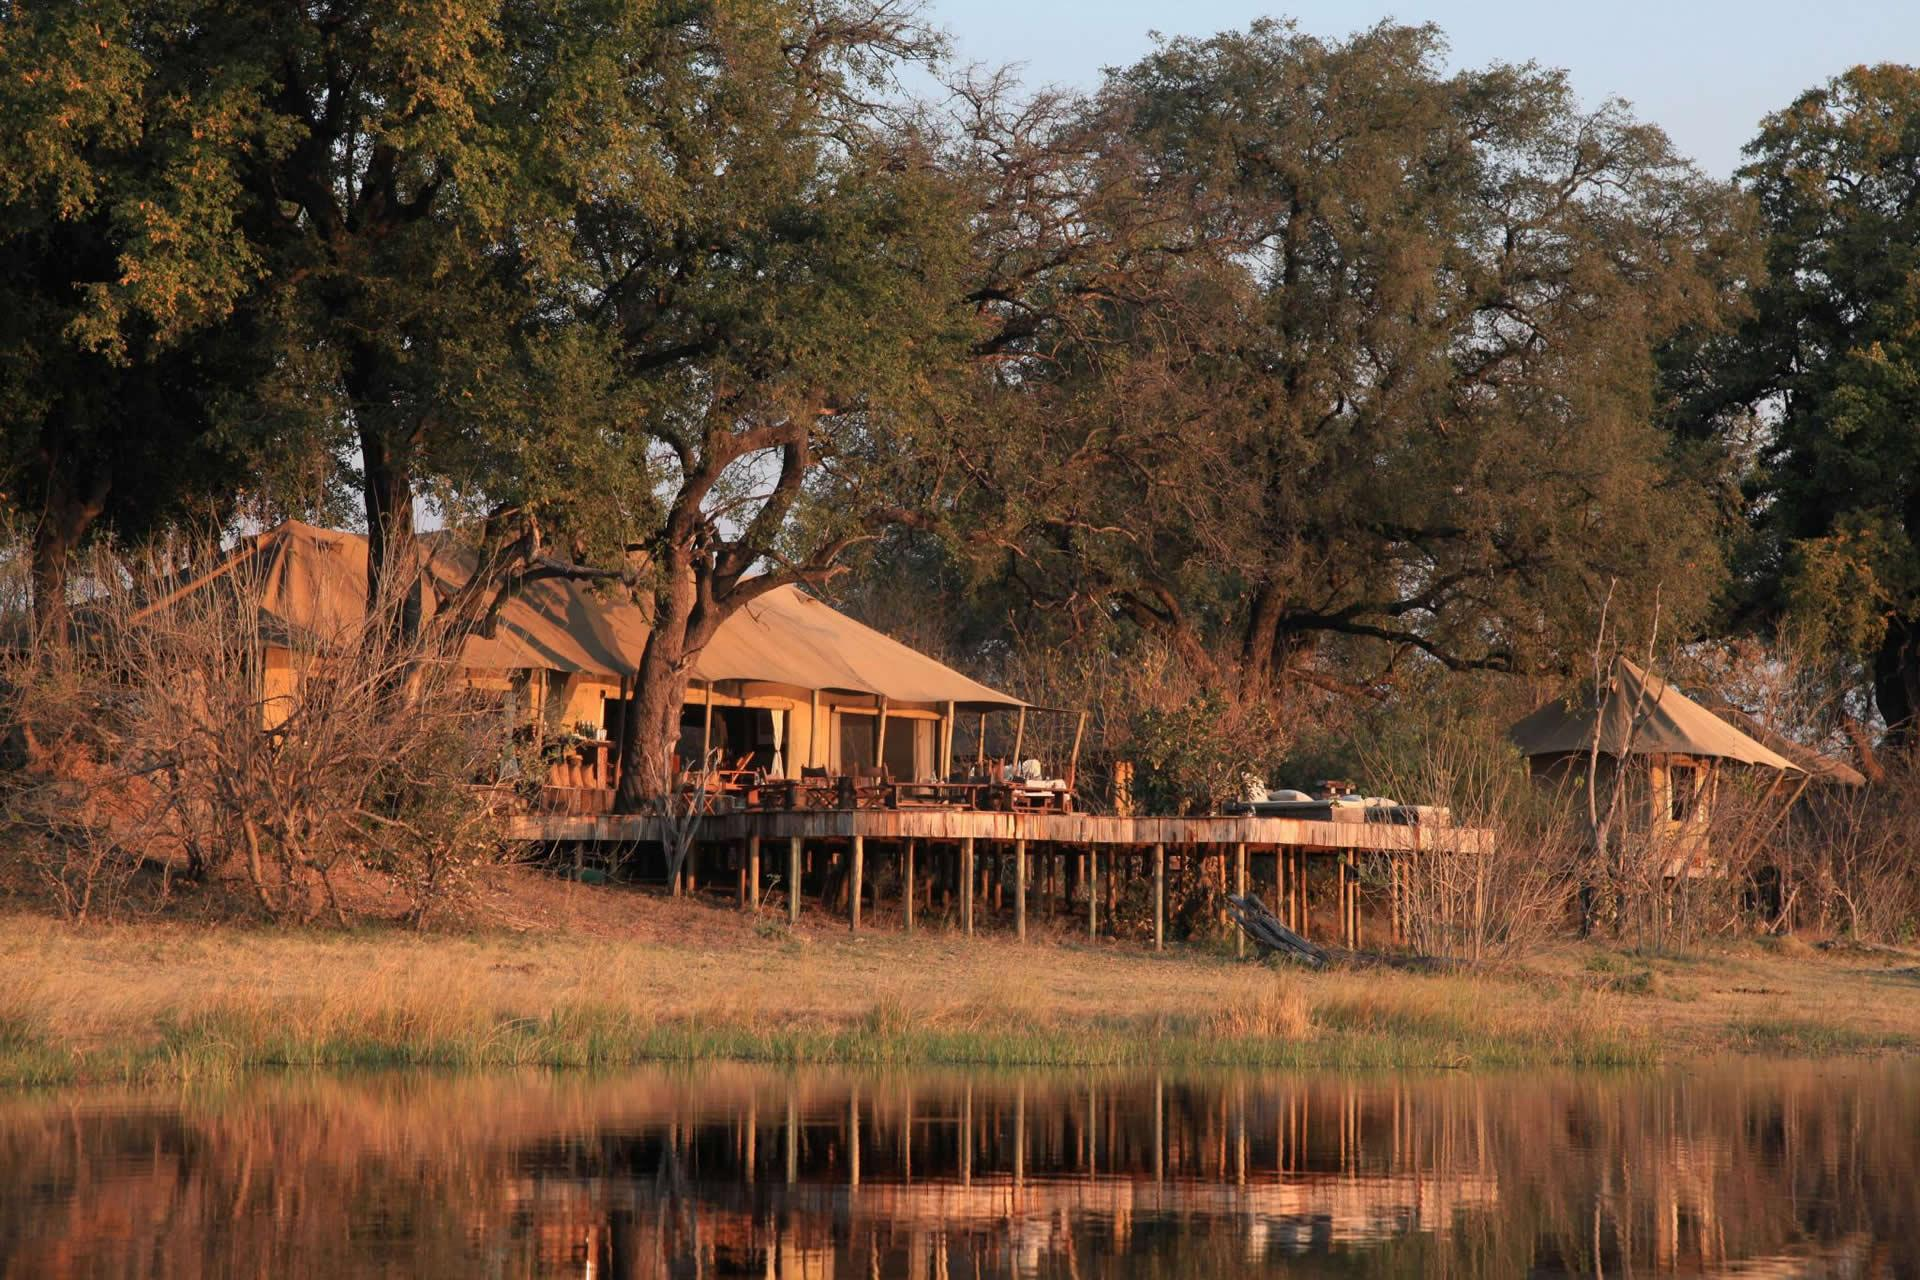
\includegraphics[width=\textwidth,height=0.8\textheight]{3.jpg} 
\end{figure}  

\newpage
\section{渣男}
\begin{quotation}
  2022/11/4
\end{quotation}

其实有一个阶段,我是不喜欢sm的,甚至排斥它。它在我眼里,是一幅画面。
一个三四十好几且有妻子和娃的男性与皮肤白皙且柔嫩的女生衣不遮体的近距离接触。
你也有自己血缘上的父亲,你也有自己血缘上的母亲,你却做着这种事情。这就是我大概两年前所理解的sm。

其实有的时候脑子比眼睛重要,通过别人的一举一动和一两句话就可以判断个大概。
可惜这么好的东西,很多人都没有,我没有针对谁,指责谁的意思,当然,在这个群体里,也包括曾经的我。    
我曾斟酌过渣男的手段,个人认为渣男都是筛选性挑选女生渣的,他们选择挑傻白甜和愚蠢的女生渣。聪明人他是不想浪费时间的。
所以看不清楚人心没关系,我们要做的是把自己的智慧提升上来,你就会发现,在你的世界里,根本没有渣男。所以这就是为什么,我们要多读书。

很久以前,流行的一句话:“我读书少,你别骗我”就是因为你读书少,才给了别人骗你的机会,让渣男有机可乘。所以我说要提升自己的内在价值和认知。
聪明的人,骗子和渣男不敢靠近你,他们为什么要挑一个这么难控制的人下手,这样你就不会给他带来任何好处。
他有渣你的功夫,他能去渣十个二十个蠢女人,他能从他们身上捞到的钱和色多的是,为什么要专挑一个有才学,有智慧的女人下手?这是有极大成本的,
所以说渣男很聪明,他会选择性的渣。就像电信诈骗专挑那些老年人渣,不懂常识的人渣,或者挑没脑子的人渣。所以蠢女人就是渣男收割机。
这就是为什么你觉得你有被渣体质,是老天在提醒你,该提升自己了宝宝。

所以我觉得这个世界上的本质就是改变自己,但是改变自己是一个很难的道路。
但是我知道,我改变自己的过程中,我身边的渣男会越来越少,甚至会消失殆尽。
所以说越艰难的道路,越要勇往直前,因为在这条路上,你收获的朋友质量都会很高。
同时这条路也是你筛选朋友的一种方式。

\newpage
\section{启蒙}
\begin{quotation}
  2022/11/5
\end{quotation}

朦胧的黄晕将整个天边悄然笼罩住,那也许是我第一次写属于自己的文章。大概是春节的前一段时间,各家灯火通明,都撸起袖子以更好的姿态来迎接新年。
母亲在厨房忙碌,像一只刚上岸的螃蟹,一双手,两只脚的身体构造完全利用成了三头六臂的效果。其中个中滋味只有她才能懂得吧。
我饶有兴趣地搬来姐姐的电脑,临时却不知道玩什么,不知是哪股力量吸引着我,使我不由自主的打开电脑备忘录,开始写起文章。这是首次,也是启蒙。
仿佛自己置身于天空之城,像是做了一场梦,一切都是那么的不真实,仿佛羽化而登仙,心灵的充实让我感觉身体也轻飘飘的。
写作的过程中,我不知未来还会有一首诗,它和我的幻境是如此意境相通。我才更深刻的理解李白笔下的《梦游天姥吟留别》。
但表达的情感和含义是不同的,这里仅仅指意境相通。

我擅长写随笔,我时常思考,如果给我一个题目,我还能否写得出来呢?
我打算尝试一下,尽管写命题作文对我来说可能有点困难。但要尝试和挑战,哪怕这样的生活不够安逸。
通过这一年的挣扎,痛苦,思索,我得出了一个结论:我不适合在安逸的情况下学习和生活,安逸使我浮躁,焦虑,同时也会产生许多不自然,
不现实的看法和念头。我的生活应该是有挑战的,有提升空间的,精彩的。它应该是这个样子的。至于这一年当中的安逸,就当作修行了吧。
我一直觉得,那些年纪轻轻就居家做功课的,没有社会经验的居士,应该早已与社会脱节了。
他们的生活太安逸了,他们念经读书所产生的见解,或多或少有些不成熟,没有经历过苦难洗礼的居士,他又怎么会生起众生皆苦,怜悯和救渡众生的心呢?
他所理解的只是在生活中虚幻的,不存在的地狱,所坚信的都是没有科学依据的六道轮回。
还有一些吃素的居士和僧人,我很想知道,他们的清规戒律是不是一种束缚呢?
会不会延续了我国封建时期的一些令人觉得痛苦和无趣呆板的制度呢?试问让他们去持守一些违背人本性的律法,这真的是好事吗?
我的问题很多,想知道的事情也很多,此生听闻和深入研究各种国家的文化,律法,风俗和文明,我觉得今生自然没有遗憾的事情了。

别人都在家里伴着淅淅沥沥的雨声睡一个美容觉的时候,我行走在蒙蒙细雨里,仿佛身体越来越轻,越来越单薄,思索着不寻常的问题。
这个思考该如何表述出来呢?这对我来说,有点难度。但是我应该试试。

\newpage
\section{天才在左,疯子在右}
\begin{quotation}
  2022/11/6
\end{quotation}

我曾读过高铭的书,其中有一篇记录了作者和一个将世界上发生的一切事情都以为是自己笔下的一个情节的精神病患者。
包括作者和他在一间小黑屋里谈论他的作品。一切都是情节,那么他是这本书里的主角。我初次读到这个情节的时候很宁静,并没有震撼,也没有新发现。
直到今天重新品读,我才明白,原来我和那位精神病患者是如此相像。我有些兴奋了,我在他身上找到了共鸣。
我也经常会思考这样一个问题:这个世界是不是我自己的?
我是这个世界的中心点,我是绝对的主角,至于家人,朋友,伙伴,他们都是一个**不足道的配角,随着情节的发展,他们随时都有可能离开我。
用通俗的话来说,他们随时都会领盒饭。所有事情的发生都是具有它自身的“道”。而“道”则为我一个人服务。
我知道这样想,太过于自我中心主义,也许还会夹带着点自私。但是我依然要勇敢起来,勇敢面对这个现象和精神世界的变化。
我不知道别人会不会这样想,到目前为止,我只发现了一个精神病患者和我曾思考过的事情很相像。
为了打败自己的特殊性,为了寻求共鸣,我会继续留意和寻找这样的人。
这个思考在这段时间频率比之前高了许多,也就是在今天,我竟然重新品读了《天才在左,疯子在右》,不知究竟是哪股力量推动我面对它,
我只觉得这很巧合,也很神奇。

也许这仅仅只是自己的一个妄念吧,狭窄的认知令我想不出来事情的缘由。
这会不会和自己的内心投射有关联呢?可惜我文笔平平,道不出傍晚时候上帝在我耳边的喃喃而语。
讲不清心中所想,说不出外界的丰富和浪漫。

浪漫忠贞不渝,圆满生生不息,晕红的脸颊和发涩的眼睛是黄昏的悸动,也是说不出口的穿越时空的暗恋。

\newpage
\section{无病呻吟}
\begin{quotation}
  2022/11/6
\end{quotation}

窗外车辆川流不息,天空云团变幻莫测,夕阳闪耀着它独特的光芒,因为这是唯独它才有的。
行走在熙熙攘攘的人群里,竟一点烟火气也感受不到。心灵仿佛已经被世俗所包裹,失去了原有的天真和活泼。
它变得不敢向外界表现出最真实的情感,它变得善于粉饰自己的感受,它经过逐渐的累积和反刍,开始变得麻木。

这并不是一个矫情的说法,也不是一种奇异的感受。这是已经生病的群体普遍的感受。
他们没有办法消解这种感觉,只能等待更猛烈的躯体症状。
像是苏格拉底等待那一杯毒酒,像是已经被架在十字架上的耶稣,他们甘于命运,甘于被折磨,实际上这是一种豁达和豪迈的心态。
他们认为人早晚要离开这个世界,乘着一轮婵娟前往另一个世界,那么早一点或者晚一点又有什么值得执着的呢。
所以这个群体散发着独特的魅力,那就是面对任何事情不骄不躁,没有任何感受。这种现象俗称:彻底麻木。

我从林奕含女士口中得知,现代文学系学生崇尚抑郁,将抑郁当成毕生追求之事。
这样来讲,也就可以理解了。不仅是文学系学生,小学生也没有落后,他们扬起‘抑郁’的旗帜,并做出伤害自己的行为。
这种举动在真正患病的人眼里,是多么的无耻和可悲。
这种行为也在无形之中给这个群体制造了许多麻烦,凡是有人说他抑郁了,他生病了,大家就都会以原来的看法和印象来看待这个病,即抑郁就是无病呻吟。

举一个例子,这种情景就如同我们孩童时期听到的“狼来了”这个故事一样。
当一个人讲自己抑郁的时候,会有人相信。当这条路走的人多了,风气被假意者污染了,这个群体沾上了污点,大家听到“抑郁” 时,便开始不屑一顾。
从此抑郁就转化成脆弱,玻璃心,矫情做作的代名词。

对于这个无形发生,我很难过。他们不是脆弱,相反,他们是坚强。他们比普通人要坚强很多。
他们日复一日地对扛着病魔,像西西弗斯般倒下,爬起来,再倒下,再爬起来。他们进入了一场可怕的循环,却仍然没有退缩。
哪怕病魔逼着他们放弃自己的梦想,他们为了对这个世界保持乐观与信任也在所不惜。
人们常说,西西弗斯推大石,不过是我们日复一日的工作生活,即从工作岗位到家这样两点一线的生活,但对于我来说,这种解释还不足够。
西西弗斯应该被精神化,它是一种风雨无阻的坚定,它是一种可贵的坚持,它是一种看透世间伶仃仍然不放弃的一种品质。
因此用西西弗斯来形容抑郁症群体毫无违和感。

虽然此刻的自己又累又饿,但是就想就这白天的感慨多说几句。

\newpage
\section{立场}
\begin{quotation}
  2022/11/11
\end{quotation}

很晚了,依然想就着现在的感想多唠叨几句。

我真的不是一个看过许多书的人,有一些人评价我的文笔好,如果对方是出于善意,我会感激不尽。
也有一些人评价我的文章东拼西凑,毫无逻辑感。我虽会有些失意,但更多的是急促感。我知道自己在对自己情绪的掌控方面,还有很多提升空间。
而此刻不修心何时修呢?这正是修心最好的时候。
面对别人褒贬不一的评价,我是否能够淡然处之,平和对待;
面临一些人的冷言冷语,我是否能做自己;听到别人的夸奖 我是否能戒骄戒躁,
为了更好的表达出自己的想法而选择此刻不发言。有些时候,我真的觉得自己有些词穷,因为一个词,我会斟酌良久。
可能是因为自己执着和要强的性子,不允许自己出现一丁点差错。否则会陷入深深的自责当中。

近期,我的心比从前浮躁了许多,也只有在写作和运动时,自己的心境才会转变。
我这段时间不停的去面对新的人事物,我无法控制自己的潜意识的运作,好像我的一切心理和行为都在围绕着潜意识而运转。
我能不能不听它的话呢?我有时候会想。在一个紧张和焦躁的心境,我只能完全听从潜意识的摆布,无法去倾听自己内心真正想要的是什么。
仿佛只有在冥想和写作的时候,我才会逐步趋向最真实的自己。

我听母亲讲,姥姥在世的时候曾患有一种极其痛苦的病,叫做肺心症。我最近常常思考,一个痛苦到极致的病人,他有没有权利去结束自己的生命。
他有没有放弃的权利。如果一个病人连对自己的生命都没有办法掌控的话,他实在算是一个可怜人。
我曾遇见一个患有抑郁症的朋友,她跳楼的那天不幸地被救治了,我明白医生救治她,是医生的天性。人做出自己天性使然的事情,有什么错呢。
只是世界上有些事情根本没有对错,主要看到底是站在谁的立场上了。虽然我的潜意识告诉我,希望她活下去。但是理性的我却希望随她去吧。因为她实在太痛苦了,因此在这样的情况下,她有权利决定自己的去留。
曾拜读过《天堂旅行团》,其中一个癌症晚期小女孩经常围绕着他的叔叔转,原因在于一个简单的愿望:看一场偶像的演唱会。
当然这只是一种浅显的解释,其中无言深意只有我彻彻底底读完了这本书,我才会明白。
一个自身患有严重疾病的女孩是希望叔叔活下去,希望他不要放弃生命。
女孩还没有见识过世间万般精彩,她的生命不长了,她希望叔叔能够活下去,替代见识她没有见识过的繁华。

这又是另外一种说法了,生和死从来都不是一个人能够决定的事情。

生,不是我们能决定的事情。死,这个决定更与我们无关。因为家人常常牵挂我们,他们会成为我们无法摆脱的羁绊。
还有一种比较高级的说法,有一些人会把自己的人生当做一场游戏,他可以决定这个游戏的开始和结束。
一个游戏而已,不想玩了就关掉电脑,何必留恋一个虚拟游戏当中的家人、朋友。
在很多人看来,这是把人生当成儿戏,这是一种不负责任的念头。
但是,谁又能证明我们的人生不是一场游戏呢?就连金刚经中都提到过:"一切有为法如梦幻泡影,如露亦如电"。
但是我们过于留恋和惦记游戏当中的人,于是便走不出游戏了 。只能无力地看着家人、朋友一个个离去。

\newpage
\section{意义是什么}
\begin{quotation}
  2022/11/12
\end{quotation}

我自从懂事的时候开始,就踏上了寻找意义的道路。
我喜欢思考,在家人和朋友眼中,那些枯燥的哲学问题是没有必要谈论的,不如想点实际的。
我有的时候也会反省自己,是不是我的生活有些安逸和清闲,让我有时间去思考这些问题。
其实不然,我忙起来的时候,也会因为某些话,某些情景,某些光景而受到触动,引起思考。
就像和家人看电影,我是最容易看哭的那一个。想到"出师未捷身先死,长使英雄泪满襟",在路边哭的像个受到巨大委屈的孩子。
我的性格、心境、情感都很柔软。我的柔软也许是没有锋芒的那一种。

其实我在任何时候都会思考一些奇怪的问题,做饭时瞥见窗外隐隐约约的绵雾,露水荡漾在树叶上,好似闻到了我的黑暗料理,便向下滑动起来。
此刻我已经觉察到自己已经陷入发呆的情景中,我能够看到"我"在做什么。
仿佛觉得身体不是自己的,我不知道"我"是谁,我突然很想知道自己是谁。还有一种情境,每次我看到蝴蝶的时候,我几乎都会想起庄周梦蝶。
我的头脑里又会冒出这样的问题,我到底是谁。我是做了一场长长的梦,一直没有醒过来吗?

这些问题思来想去,又会变得更豁达。人生如同一场梦境,在梦境里,我们不妨去攀一座山,追一个梦。
我们也可以选择"摆烂"的生活,就像诗人陶渊明,追求自己的生活品质。就像大冰笔下的摄影师阿让,他极力追求属于他的梦。
但是"摆烂"不是不作为,而是顺其自然。这世界上一切事物都有属于它自身的运行轨迹,我要做的只有与生活融为一体,而不是对抗它。
就像我的情绪,我之前说错了一句话。不要与它打持久战,应是静静的邀请它来喝杯茶,坦然应对。

这些是我在写作的过程中,产生的一些感悟。即通过我的体悟,自发孕育出来属于自己的"道理"。
这些可能是属于自己的"心灵鸡汤",但是它和网络上的一些鸡汤是有些不同的。尽管网络上的心灵鸡汤也是劝人向上、努力。
可是我们是一个活生生的人,是感性动物。我们不可能做到绝对理性,既然是感性动物,就会被情绪控制,在这个时候,心灵鸡汤就没什么效果了。
谁能在一个崩溃的人的耳边洪亮地说你要努力,你要加油呢。这就好像对一位双腿残疾的人说:"你站起来跑一跑就好了"。
仿佛是对一位失目者说:"你睁开眼睛看看,这个世界很美"。这些例子的结果和网络上的一些心灵鸡汤的效果一般无二。

我只是想表达,如果过度将某些道理奉为圭臬,对事物缺乏判断和理解能力,失去分析其他立场的能力,
活在鸡汤所营造的美好幻象中无法自拔,只会病入膏肓而不自知。
但是自己总结出的"鸡汤"就不一样,它是我们切身实践过之后总结出来的。

\newpage
\section{嗅觉的真理}
\begin{quotation}
  2022/11/15
\end{quotation}

现在是晚上七点十七分,当我写下这个时间点时,自己的心仿佛被重新洗刷了一番。
我随着沉重的音律安稳地走向远方的灯塔。
是什么使我那么笃定地相信这就是灯塔的方向呢?其实按照之前自己的唯心主义,我会认为是情绪主导者我的一切。

曾经有这样一位前辈提点我:“蚂蚁一贯靠嗅觉来找到它心仪的食物,它处在二维的世界里,我们在蚂蚁的身后放了一块蛋糕,
他的眼睛看不到这块蛋糕,它依然能找到蛋糕并津津有味地吃掉,这时候就是嗅觉在它寻找东西时发挥着重要作用”。
当我正在思考其中的妙趣时,前辈蓦地问我:“那你知道,我们人类是通过什么来确定我们通往梦想之路的方向吗?”我迟疑地吐出两个字:“情绪”。
看他的语气,我的回答明显正确。后来我再次回想,为什么是情绪呢?似乎只有这一个答案符合题意。
当我选择的道路给我带来的是痛苦和纠结时,我知道,这和标准答案显然背道而驰了。
但是在这个时候,我该不该放弃呢?我暗自思忖,似乎不应该将自己的初步结论奉为标准答案,我应该再通过其他的角度分析前辈的忠告。

也许他的意思是当我们做任何一件事情都用乐观、喜悦和感恩的心态去完成的时候,那么我们就离成功不远了。
这种所谓的成功学,并不能够吸引现在的自己,然而原来的自己(十五岁)的自己,将成功学的理论奉为最重要的理论。
那时候的自己狂热地追求所谓的成功,经历了一系列磨难和纠结之后,我不再相信这些,我甚至鄙视。
但是我不能因为现在的人生阅历多了一些,就将从前的一切寻找和印证全盘否定。
人的成长历程就像一座金字塔,需先将底层建筑打好基础,才能进行进一步的建筑。
在底层建筑的期间,我们会感到迷茫痛苦,不知前路的方向。由此会因为某一个理论或者某一个人拯救了自己而将其奉为神明或雕像。
当我们真正强大起来的时候,回过头来审视曾经的自己,会觉得原来的自己傻里傻气。
其实不必自责,不必羞耻,这是人的成长道路上必经的一站。

从小到大,我经常会自责和自我反省。但是道理好像都已经烂熟于心,却始终没有勇气接受自己,拥抱自己。
我承认现在的自己勇气不足,导致许多自己想做的事情至今没办法完成。
也许在将来的某一天,我会后悔自己没有勇气去做出正确的决定。今天的文章写的相对来说比较流畅,至少和前些天比较显得流畅一些。
我曾反复思考过这样一个问题:为什么我的思考总是受到限制和堵塞。有什么方法可以让它一帆风顺地进行下去呢?
这就像一个瓶颈期,无论做出何等努力都无法突破它。

\newpage
\section{美梦总是很短暂}
\begin{quotation}
  2022/11/19
\end{quotation}

前两天夜里两三点钟起身时摔倒在客厅的走廊。胸闷与目眩笼罩我的身体。
但那天确实滴酒未沾,前一秒还清醒的很,后一秒便沉浸于困意的漩涡中。
我记得曾经的张老师,我对他几乎不存在什么执念了,他只是我人生中的一束灯光。在无穷的黑暗中,那一丝灯光才显得那么重要。
这束光照射在少女常用的小镜子上,通过镜子反射照进天花板上,散落的光芒暖了我的心房。这是多么震撼的情景。

在我心里,他是绝对不容质疑的完美无瑕,仿佛是一个瓷娃娃,制作过程中不允许出现任何纰漏,否则就会失去它原有的质地。
或许,我还是一个灵魂从未长大的"孩子"吧。我心中的雕塑仍然屹立不倒,它成为了我在每一个孤夜难眠之夜的思念对象。
我知道那仅仅是我心中的一个艺术,它是理想的海洋,是幻境的浮云。而我,是臣服在艺术之下的沉默的羔羊。
这也许是我不成熟的地方,它是我理想主义的境地,是我乌托邦的世界。

张老师的嗓音按照现在的流行词来说,是一种历经沧桑的烟嗓。他曾弹唱"阿拉斯加海湾"、"琴师"等等。我原本听过这些曲子,但也只是随意听听。
直到我听见他的弹唱,仿佛如听仙乐耳暂明。这些曲子因为他的歌喉,在我心里便竖立起它们存在的意义。
当我知晓他离开我们时,宛然失去了一个排遣内心疲倦失意的场所,宛若失去了一个故友。
我了解事情的大概情况后,心中虽有些不舍,但更多的是庆幸。
作为一个冷静的粉丝,我担心他遭遇网暴之后的心境,后来想想,我发现自己担忧的有些画蛇添足。
他能有这样的思想,证明他从来不是一个软弱的人。如今倒平白增添了些许平和及心安。
原来心系一个人是这样的感觉,我希望我的日常起居和他同步,倘若自己的心境和他相似,我会多么荣幸。

我愿意成为他,哪怕经历一遭他的痛苦,承担下他的罪过,我也义无反顾。
我羡慕那些精神世界丰富多彩的作家或者画家,即使他们不受人理解和支持。

我的梦境里曾反复出现的场景:在萧瑟的秋风中,在银黄色落木的掩映下,在枯叶蝶无声的哀鸣下,一位身穿黑色风衣之人坐在长椅上,
拿着一本徐志摩的诗饶有趣味地读着。我不敢靠近他,只能在礼貌的分界线外饶有兴致地看着。
蓦地一只蝴蝶飞到我的眼前,调皮地挡住我的视线。这时候我才真正醒来,我不知为何,此梦境总是频频出现在我的脑海里。
我没有太多的精力理会它,直到我真正体悟到此梦境蕴含的无言深意。
原来"它"的影子一直在我的脑海里,影响着我,鞭策着我,激励着我,如同嗅觉一般引领我行走在正确的道路之上......

\newpage
\section{受伤}
\begin{quotation}
  2022/11/22
\end{quotation}

晚风掠过珠窗轻柔地吹拂我的发丝,清逸谧静的琴声悠扬回荡在空气中,往日的情景竟如潮水般向我涌来。
心中万分忧愁,提笔却寥寥几行。当真觉得自己是一个自私的人,轻言放弃生命,却不顾他人感受。
这几天我如同林黛玉一般多愁善感,泪水经常义无反顾地浸湿衣衫。蹲在马路上,脸上没有涂抹任何脂粉,却如同一个露出棉花的布娃娃。
我不曾遭受巨大的委屈,仅仅觉得后悔莫及。

自从与一个从天而降的礼物开启美好的际遇之后,我便养成了运动的习惯。那天的运动量大且高强度,我做完最后一个动作后累的瘫在瑜伽垫上。
汗水像一滴又一滴的鲛珠,豪迈地洒在我的脸上,锁骨上,额头上。布满了衣裳,抚慰了心灵。母亲一瘸一拐地缓缓走过来为我拭去汗水。
那一刻,我的内心是崩溃的。更多的是感动,它就像冬日里的一抹阳光,温暖的阳光照射进我的内心。
我崩溃的原因是母亲身体不好,我怕母亲离开我,如果母亲去世了,就没有人在我运动的时候为我擦汗了。
我知道没有人会像母亲这么细心地呵护我,我十分害怕,十分不舍,情绪便像火山一般爆发,喷射出一股热腾腾的泪水。
母亲笑着打趣我,说我多愁善感,说以后再这么哭,可就给我找哭活去了。谁知我的内心是多么无助和恐惧。
上天善嫉,原本幸福平静的生活被他打破,于是碎成了一地的泪珠。
前一阵子母亲因为急匆匆地赶车不小心摔倒了,这时候母亲打的第一个电话不是我,而是长姐。可能我年纪尚小,并不能帮上什么忙吧。
于是长姐买轮椅,买拐杖,在母亲所在的医院照顾她,在手术室外焦急的等待结果。当时正值疫情,病号身边只能陪伴一个亲属。
而此刻在家的自己,却很自责,不能时刻陪伴在母亲身边为她侍疾。可能将来的某一天,我会遗憾没有在母亲最难熬的时候陪着她身边。
许多事情,只有无奈的份,却没有挽救的机会。

今天我受到了他人无意中的伤害,心情复杂失意,便独自坐在窗前掩面哭泣。
母亲在一旁询问和劝说,字字句句都是她的真情实感,我却听不进去。也许母亲在我的眼神中看到了绝望,她拉着我的手说:“姑娘,妈离不开你”。
听到这句震撼我心的话,我哭的更厉害了。我深知自己这很多事情上无能为力,甚至不能理解父母的苦心,可是他们依然对我死心塌地。
一切都为我着想,他们是这世上对我最好的人。
母亲说过,她的孩子生病的时候,她的心仿佛在滴血,倒不如这病痛降临在她身上。这是多么震撼的一句话。

我至今印象深刻。她也是穷困的家庭里长大的,然而在没有受过多少教育的家庭里,竟生长的如此伟大。
我始终认为,母爱是高尚的。
即使在这个世界上,母爱的高尚并不是一件新鲜的事情,大多数的母亲都爱自己的孩子,但是我依然觉得,这种情感是崇高的,是不可比拟的 。
我宁愿要那种“上有老”的沉重,也不愿以永失父母的天伦亲情,去换一份卸却沉重的轻松。
我觉得父母健在是一个美好的词,它对于芸芸众生来说,是一种可贵的幸福。
母亲如同河水一般养育一方鱼群,母亲是我的河水,我就像鱼儿离不开河水一样离不开她。我不曾想过我们分离时,我会是何等的崩溃和绝望。

只能在此祈愿,母亲能够平平安安,万寿无疆。

\newpage
\section{病发}
\begin{quotation}
  2022/11/26
\end{quotation}

烦,无休止的烦躁。仿佛自己戴着灰色的眼镜在观察这个世界,目光所见之处皆是无尽的黑暗。
走在熙熙攘攘的人群里,孤独感更加肆无忌惮。有可能是曲唑酮的缘故,困意像藤蔓一般螺旋式上升到头脑。
大脑里一直反复浮现的画面,使我不得安心。想到自己上学的时候脑子笨的不得了,甚至软弱,胆小,自卑,焦躁,自尊心非常强。
一系列贬义词都成为了我求学时期的代名词。面对一些人的言语攻击,我无法回怼。因为在那个时候,我的面部肌肉会抽搐,我甚至说不出来话。
事后我会责怪自己,其实不必责怪的。倘若我的面部肌肉不会抽搐,我依然不敢回嘴。

也许我真的不是一个合群的人吧,我上学的时候人缘不好,无论小学初中,体育课中的自由活动是我最难熬的时候。
因为我不愿意和别人一起玩,没有任何原因。如果深究其缘由,我想应该是自卑和内向吧。
在那个时候,我从来没有想过向神明申请批准人间长假,无论我多么辛苦,心理承受了多大的委屈和压力。
我记得考试前期,我整理错题本整理地有些晚了,睡得太沉,早上甚至没听到闹钟的声音,因此起晚了。
我急匆匆地赶到学校之后,结果等到的却是一张扣分表,那个男老师眉头紧锁,询问我的名字和班级。
我一下子害怕了,是我自尊心太强的缘故,我恳求他不要扣分,我真担心我当时膝盖一软,便向他这种人跪下。
但是我当时竟然有这种想法,我真替自己感到不值和羞耻。
于是他让我去求我的年级主任,我当时没有一刻犹豫,内心的恐惧已经覆盖住了羞耻,我顶着红彤彤的脸去求年级主任。

幽暗的草丛里生长着一束玫瑰花,它的身体上布满了刺,我的记忆还停留在草丛里,每当我想起它来,我的心脏就被玫瑰花刺的痛不欲生。
试问是谁毁了我?我无力追究他人的责任,但是愤慨依旧深深扎根于心。
就像一位植物人患者,我们不知他心中所想,但是可以通过他的眼神来感受他的内心。比如挣扎,痛苦等等情绪。
我当时懒惰地躺在床上,和植物人又有何区别?我恶心想吐都懒得起身,却也只能扶着床头柜慢慢起身。
我记得那时在一所中医院,我在诊室门口依靠着椅子。医生叫我的时候,我突然发现自己已经动不了了,仿佛动一下就用尽了全身的力气。
我好像仅剩一口气了,我不想再耗费力气去看医生了,因为他开的**,对我来说都不起效果。
我走路需要人扶着,我一步一步地走进诊室,那种心力交瘁的感觉应该只有亲历者才能体会,依靠想象是感受不到真正的无力的。

仿佛处在一个老师说数学题不难,自己却解不出来的无力感中,这种无力感是精神上的感觉。而我看医生时候的感觉,是精神和身体上统一的无力感。
医生在呼唤我,我的内心在呐喊,我的母亲在一旁焦急又心疼地扶着我。我何尝不想移动,可是我根本没有与之匹配的力气去行走在冰凉的地板上。
在这个时候没有人理解我,甚至我也无法理解自己。

我是馊掉了的酸奶和浓汤,我是爬满虫卵的玫瑰和百合。我是这个繁华都市的一个庸碌人,我是不被人需要的野花。




\chapter{救赎}
改变总会是不容易的。

虽然他人的帮助会使事情变得简单起来,但自己的话,
会使自己真正成长。

而当我无数次跌倒后,依旧可以站起来时,请记得为我祝福。

\vspace{8em}
\begin{figure}[H]
  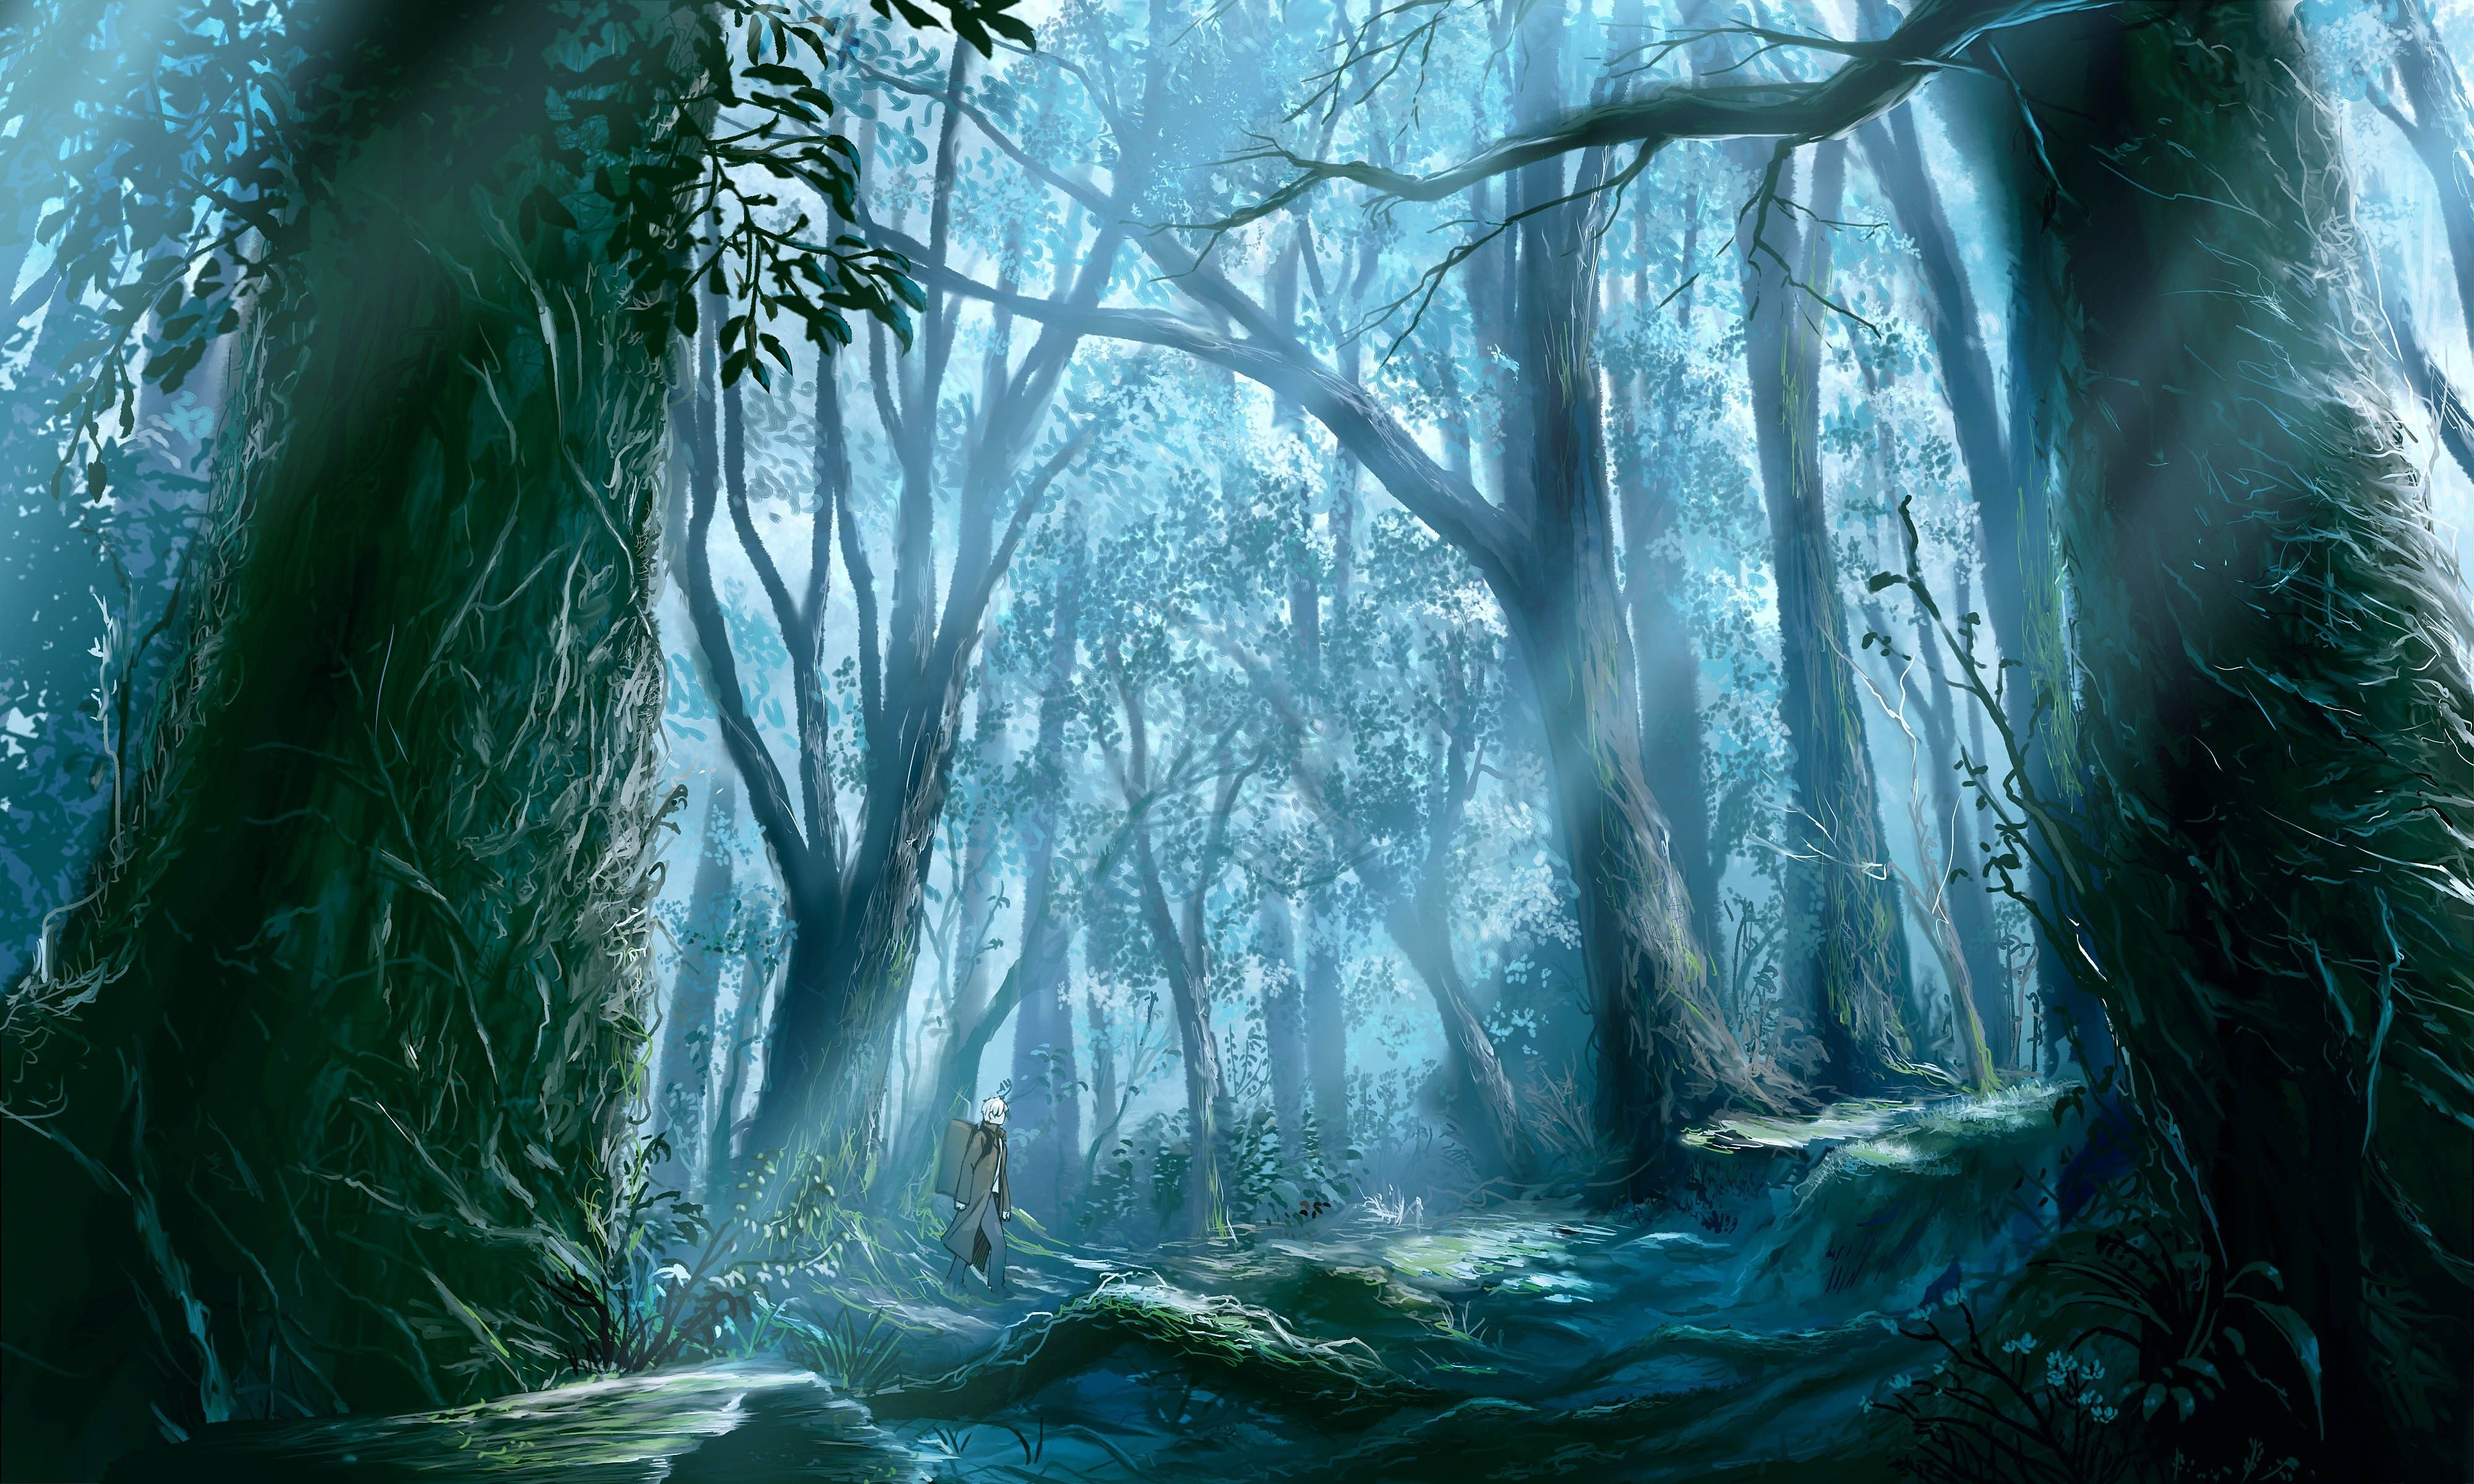
\includegraphics[width=\textwidth,height=0.5\textheight]{4.jpg} 
\end{figure}  


\newpage
\section{暗夜}
 
在长久的时间里我感觉自己像是落入到黑暗里,浑身动弹不得,
   每走一步路,感觉都要用尽全身力气才行。在一次又一次的内耗中,
   终于,有一天,我只能无奈地告诉世界,我走不动了。

   亲人朋友,包括好多的人纷纷给我了一些专业的建议,
   大概就是,我应该好好休养,还有可能我的精神上也许出了一些状况。
   我也确实感觉自己精神不是很好,内耗对于精神的损伤无比严重,
   但有些事情,我却忍不住,我想不明白,会去反复不断地想。
   
   我逐渐变得扭曲,头疼,失眠,负面情绪……

   我知道我是时候该放弃思考了,可是我的精神如此脆弱,
   一句玩笑,也可能瞬间令我窒息。
   我想通过麻痹,来获得短暂的清醒,
   可是,堕落的深渊,好像永远也看不见脚下的地面。
   家人虽然希望我能早点好起来,
   可是我已经不知道怎么样才算是好起来了……

   在一次偶然的事情中,我遇到了他……

   
\newpage
\section{缓刑加权}
小狗的各种行为,其实还是主要根据主人的喜好来定的。
在这里制定小狗的惩罚机制,也就不得不表达一下主人我的喜好。

听话的小狗无疑每个主人都是十分喜欢的,我也不例外,但是主人的决定,
有时候给小狗也会带去不可逆的伤害,这是有的主人不去注意的,或者为了自己的喜好而刻意忽略掉了。
我想当一个贤明的主人,可能这句话在更高的维度听起来很可笑,但对于小狗,我是真诚的。

缓刑加权,我觉得可以很长时间延续在你我主仆之间,惩罚的方式就是简单的打屁股。
做不好的事情加,做好的事情减,积累到十下就做一次清算。(因为积累多了小狗估计就承受不住了)

下面我简单的说一下我所能掌控的一些:

+1:早上九点之前给主人请安

-1:早上九点之前没给主人请安

+1:不经意时让主人开心,或做的事情值得主人肯定

-1:做的事情让主人不开心

\newpage
\section{关于学习}
关于学习,我觉得就像是搭积木,用小小的形状的积木,甚至可以搭出恐龙。
玩积木稍有不慎,就要重新搭建,因为你用错的某个小部件可能卡在恐龙的深处,
很令人恼火。

当然,积木的世界有一个约束,那就是:新的积木,本质上还是原来的积木所组成的。
不然那就不叫积木世界了。

至于你现在所拥有的积木,大概应该是有一些了的,但是你自己好像不太知道,
甚至于说,已经相当模糊了。哪怕是这样,我问你,你会解方程吗?你的回答也是很干脆的说谁不会。

于是你应该知道,你不管怎么看低自己,但你始终走过山路的,你不管怎样低垂头颅,也会比那些站在平地踮脚的人要高大。
而你就算是踮起脚尖,在比你走过更多山路的人眼中也不过如此。

可是,我看到你对我低垂丧气,我很生气,你对自己的要求没有什么逼数,反倒说自己什么都做不好。

如果你还是自己不清楚自己怎么了,就好好给我汇报一天天的所作所为。
因为总会有一天当你回头看你自己的汇报时,你就会突然明白自己应该怎么做了。

\vspace{4em}
在我看来,学习的前提是拥有一个坚实的心智,因为在自习的情况下,学习不再是所见即得,而是披荆斩棘。
挫折将大于收获,失败是常有时。

可是,这样的情况是出现在什么时候呢?

好像是初学者大多会有,其中无法平静地接受掉挫折和失败的人,哪怕多么天资聪颖,也最终会选择放弃。
而只有平淡的接受了自己的浅薄,并始终坚定地朝着山路前进的人,不但说他们不在会有初学者的胆怯,好像他们还变得聪明了。
至于为什么变聪明了,我大概理解为他们比较专注,这也是我最近有的感觉。




\appendix



\chapter{作业}

一些乱七八糟的作业。
  \subsection*{2023/9/22}

    \vspace{3em}
    \begin{tikzpicture}
    \draw[-latex](1,1)node[below left]{$A$}--(3,1);
    \draw[-latex](8,1)node[below right]{$B$}--(6,1);
    \draw(1,0)--(8,0);
    \end{tikzpicture}
    \vspace{3em}
    
  A、B两辆小车相对运动,A车的速度是5m/s,B车的速度是4m/s,
  最开始两辆小车相距30m,问他们相遇需要多少时间?
  \vspace{3em}


    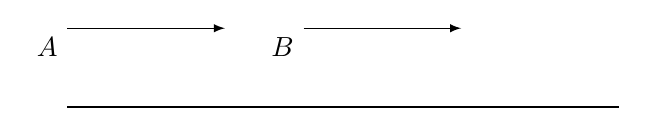
\begin{tikzpicture}
    \draw[-latex](1,1)node[below left]{$A$}--(3,1);
    \draw[-latex](4,1)node[below left]{$B$}--(6,1);
    \draw(1,0)--(8,0);
    \end{tikzpicture}
    \vspace{3em}

  当A、B两辆小车相距12m,改为同向运动时,A追B需要多久时间?


     \subsection*{2023/9/23}
     
     1、 一辆小车的速度是4m/s,
      
      (1)5秒后,小车行驶了多少距离?

      (2)30m的距离,小车需要行驶多久?
        
      (3)另一辆小车的速度是5m/s,两辆小车同时出发,
      问需要行驶多久,两辆小车行驶的路程之和是30m?

      (4)在第三问的基础上,
      问需要行驶多久,两辆小车行驶的路程之差是12m?
       
      2、帮我解释一下变化率是什么意思,速度的变化率怎么求?
        假如速度是关于时间的函数,如$v=3t$,$v=t^2$,分别的变化率怎么求?

     \subsection*{2023/9/24}
      
      1、准备一个摘抄本,
       摘抄《岳阳楼记》《定风波•莫听穿林打叶声》,
       对自己不懂的字词进行注释。
       试总结作者表达了什么样的人生态度。(要求摘抄时字迹整齐)
       
      2、写一篇英文小作文,记一件开心的小事情。(要求字数不少于80字)
      
      3、因式分解,是高中数学计算中常用的手段,如
        \[x^2-x-2 =(x-2)(x+1)\]
        \[ x^2+3x-4 = (x-1)(x+4) \]
        左边式子写成右边式子,往往可以触发化简机关,
        感受其中的特点,自学后
        试着写出 $ 2x^2 -(a-2b)x -ab$ 因式分解的结果。

    
     \subsection*{2023/9/25}
        1、摘抄《蜀道难》,注释不懂的字词,要求摘抄时字迹整齐。

        2、摘抄一首英文诗歌,注释不懂的单词短语,要求摘抄时字迹整齐。

        3、关于函数的极值,
        试求以下函数当$x$取什么值时,函数有极值?

        (1)、$ f(x) = x^2 - 6x + 9$
         
        (2)、$ f(x) = x^2 + x -12 $ %(x-3)(x+4)
       
        (3)、$ f(x) = 2x^2 -(a-2b)x -ab $

        
        \subsection*{2023/9/26}
            
          \begin{tikzpicture}
              \draw[] (4,0) -- (6,3);
              \draw[] (2,0) rectangle (6,-1);
              \draw[thick] (0,-1) -- (8,-1);
              \draw [-stealth,thick] (7,4.5) node[below right] {$F$}-- (6,3); 
              
          \end{tikzpicture}

          正在拖地的拖把可以近似的看成如图所示的几何形状,
          重量可以当成全部集中在长方块部分。
          假如地面的静摩擦系数是0.5,拖把重$5kg$,
          人在杆上的作用力为F,
          (重力加速度取近似的$g=10m/s^2$)

          (1)、长方块受到地球给它的重力是多少?

          (2)、长方块可以受到的最大静摩擦力是多少?

          (3)、假设力的方向和水平方向的夹角为$30{^\circ}$,
          当F多大时,F在水平的分量等于最大静摩擦力?

          (4)、(秘密)

\subsection*{2023/10/4}
\begin{tikzpicture}
  \draw [->] (-3,0) -- (3,0)node[below right]{$x$};
  \draw [->] (0,-3) -- (0,3)node[right]{$y$};
  \draw [->] (0,0) -- (-1.6,-1) node[below left]{向量1$(F=2N)$};
  \draw [->][thick] (0,0) -- (0,-2) node [below right]{向量2$(G)$};
  \draw [thick][->] (0,0) -- (1.3,0)node [above right]{向量3$(f=\sqrt{3}N)$};
  \draw [thick][->] (0,0) -- (0,2) node [right]{$F_{N}=?$};
  \node[left]  at (-0.7,-0.3)  {$30^{\circ}$};

 
\end{tikzpicture}

\begin{equation}
  \begin{split}G=mg,m=0.2kg \\
   & (g=10N/{kg})
  \end{split}
\end{equation}

(1)、由图,已知向量1,2,3($F,G,f$)的大小,求他们的向量和

(2)、根据力的三大定律,静止的物体所受合外力为零,也就是所有的向量之和为零,推理向量$F_N$应该是多少

\begin{tikzpicture}
  \draw [->] (-3,0) -- (3,0)node[below right]{$x$};
  \draw [->] (0,-3) -- (0,3)node[right]{$y$};
  \draw [->] (0,0) -- (-1.6,-1) node[below left]{向量1$(-\sqrt{3},-1)$};
  \draw [->][thick] (0,0) -- (0,-2) node [below right]{向量2$(0,-2)$};
  \draw [thick][->] (0,0) -- (1.3,0)node [above right]{向量3$(\sqrt{3},0)$};
  
  \node[left]  at (-0.7,-0.3)  {$30^{\circ}$};

 
\end{tikzpicture}




向量和= 向量1 + 向量2 + 向量3 

 $= (-\sqrt{3},-1) + (0,-2) + (\sqrt{3},0)$

 $=( (-\sqrt{3})+0+\sqrt{3},(-1)+(-2)+0)$

 $=(0,-1)$

 坐标中向量的加减法,即横坐标和横坐标相加减,纵坐标和纵坐标相加减。
 是不是比向量的三角形/平行四边形法则要简单的不要不要的。



 
 %\chapter{基础}
   






	
	
\end{document}
